\chapter{Построение низкоразмерных моделей при неоднородных вариациях пространственных полей}\label{ch:ch4}

\todo{2 pages}

\todo{\cite{Elizarev_2021}}

В данной главе рассматриваются особенности репрезентативного эмпирического низкоразмерного моделирования при неоднородных изменениях пространственных свойств. В контексте Уравнения~\ref{eq:blackoil} в качестве таких свойств могут выступать поля пористости и проницаемости.

На примере модельной задачи рассматривается инвариантное преобразование координат в сочетании с линейным преобразованием коэффициента диффузии $\check{\kappa} = \frac{\check{\kappa}}{\kappa} \cdot \kappa$.

\begin{align}
    \deriv{u}{\check{t}}
    - \frac{\check{\kappa}}{\kappa}
    \frac{\beta^2}{\alpha}  \kappa \deriv[2]{u}{\check{x}} = \frac{q}{\alpha}
\end{align}

В данной работе рассматривается случай малого количества областей, преобразование пространственных свойств в рамках которых можно считать однородным. В такое случае предлагается использовать аналогичных подход независимых главных компонент из Главы~\ref{ch:ch3}. В таком случае координаты не преобразуются, но для сшивки паттернов в выделенных областях используется непосредственно факт независимости главных компонент в этих областях.

\begin{figure}[ht]
    \centerfloat{
        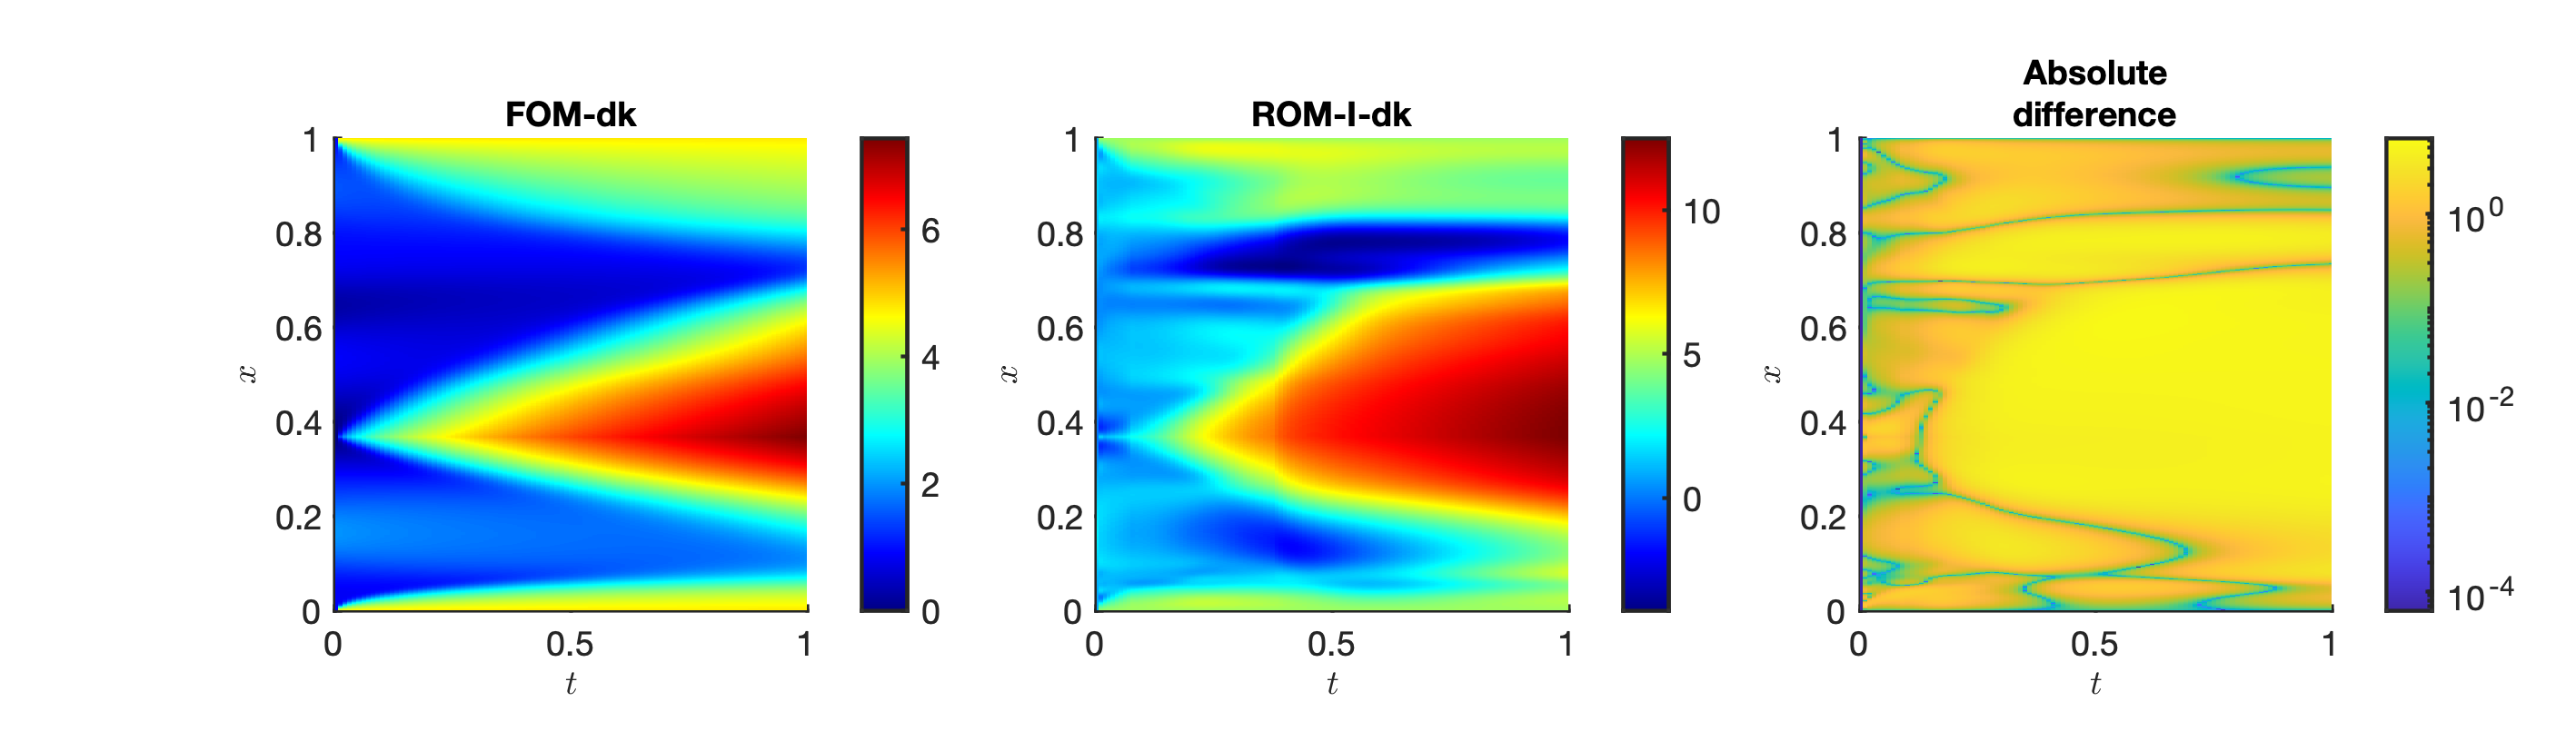
\includegraphics[width=\textwidth,trim={2.5cm 0 0 0},clip]{sci_report/images/ECMOR/11-Problem-K.png}
    }
    \caption{Использование главных компонент, полученных при некотором пространственном распределении коэффициентов диффузии, в задаче с неоднородно преобразованном распределении этих коэффициентов~\cite{Elizarev2022}}\label{fig:q-domains}
\end{figure}

\begin{figure}[ht]
    \centerfloat{
        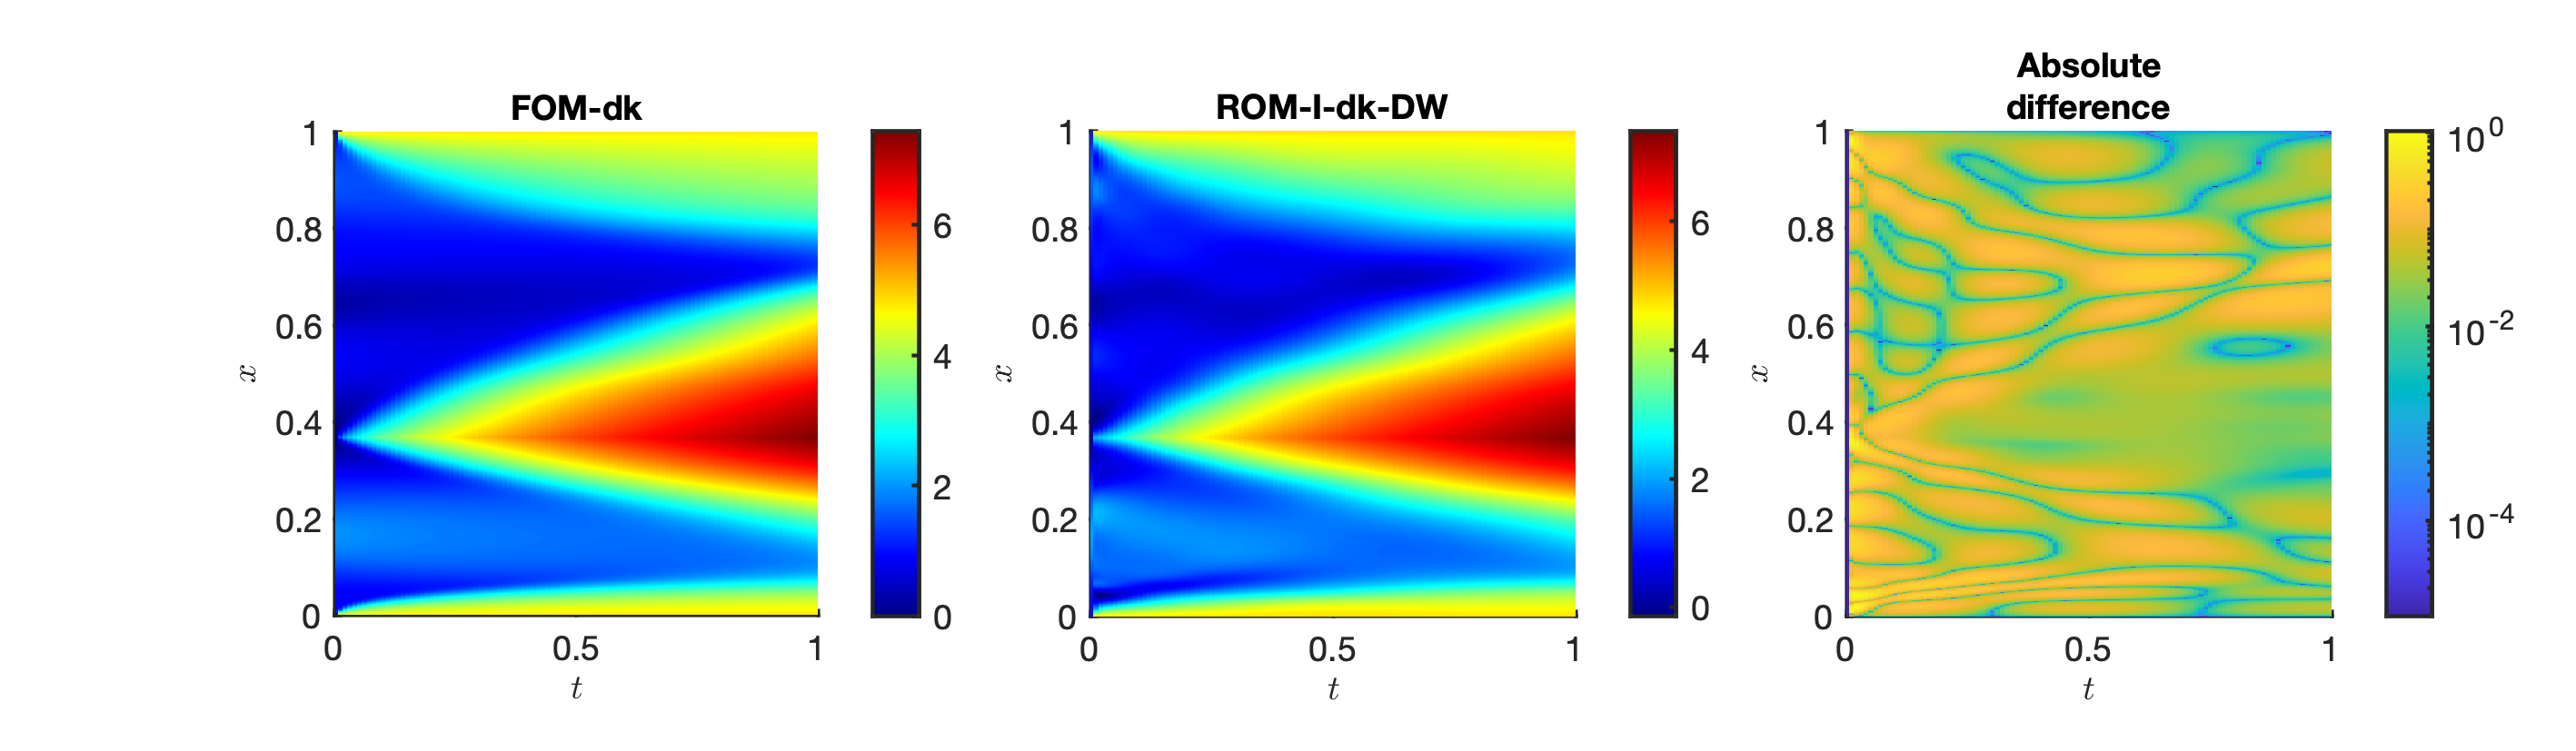
\includegraphics[width=\textwidth,trim={2.5cm 0 0 0},clip]{sci_report/images/ECMOR/15-Result-K.png}
    }
    \caption{Качество эмпирического низкоразмерного моделирования неоднородном преобразовании кожффициентов диффузии при использовании приближенных инвариантных преобразований~\cite{Elizarev2022}}\label{fig:q-non-uniform}
\end{figure}

В этой главе дополнительно отмечается, что согласованное со смещением источника преобразование координат в Главе~\ref{ch:ch3} проводилось без дополнительного учёта неоднородности поля коэффициентов диффузии. В случае смещения источника негативные побочные эффекты неоднородности пространственных свойств могут быть нивелированы малостью таких смещений и наличием в обучающей выборке численных решений при иных пространственно-распределенных параметрах для более обобщённой репрезентации.
